% !TEX root = ../main.tex

\chapter{谷歌TPU使用脉动阵列实例}

图~\ref{fig:tpu_systolic} 是一张脉动阵列运算实例的示意图。
图中对象1114就是脉动阵列。
对象1110是向量输入,也是脉动阵列中传递的数据。
它是通过激活输入经过图中方法排序得到的。
脉动阵列中的Mux列就是多路复用器的选路序号,与向量输入对应起来,就可以得到图中数据。

\begin{figure}[!htp]
  \centering
  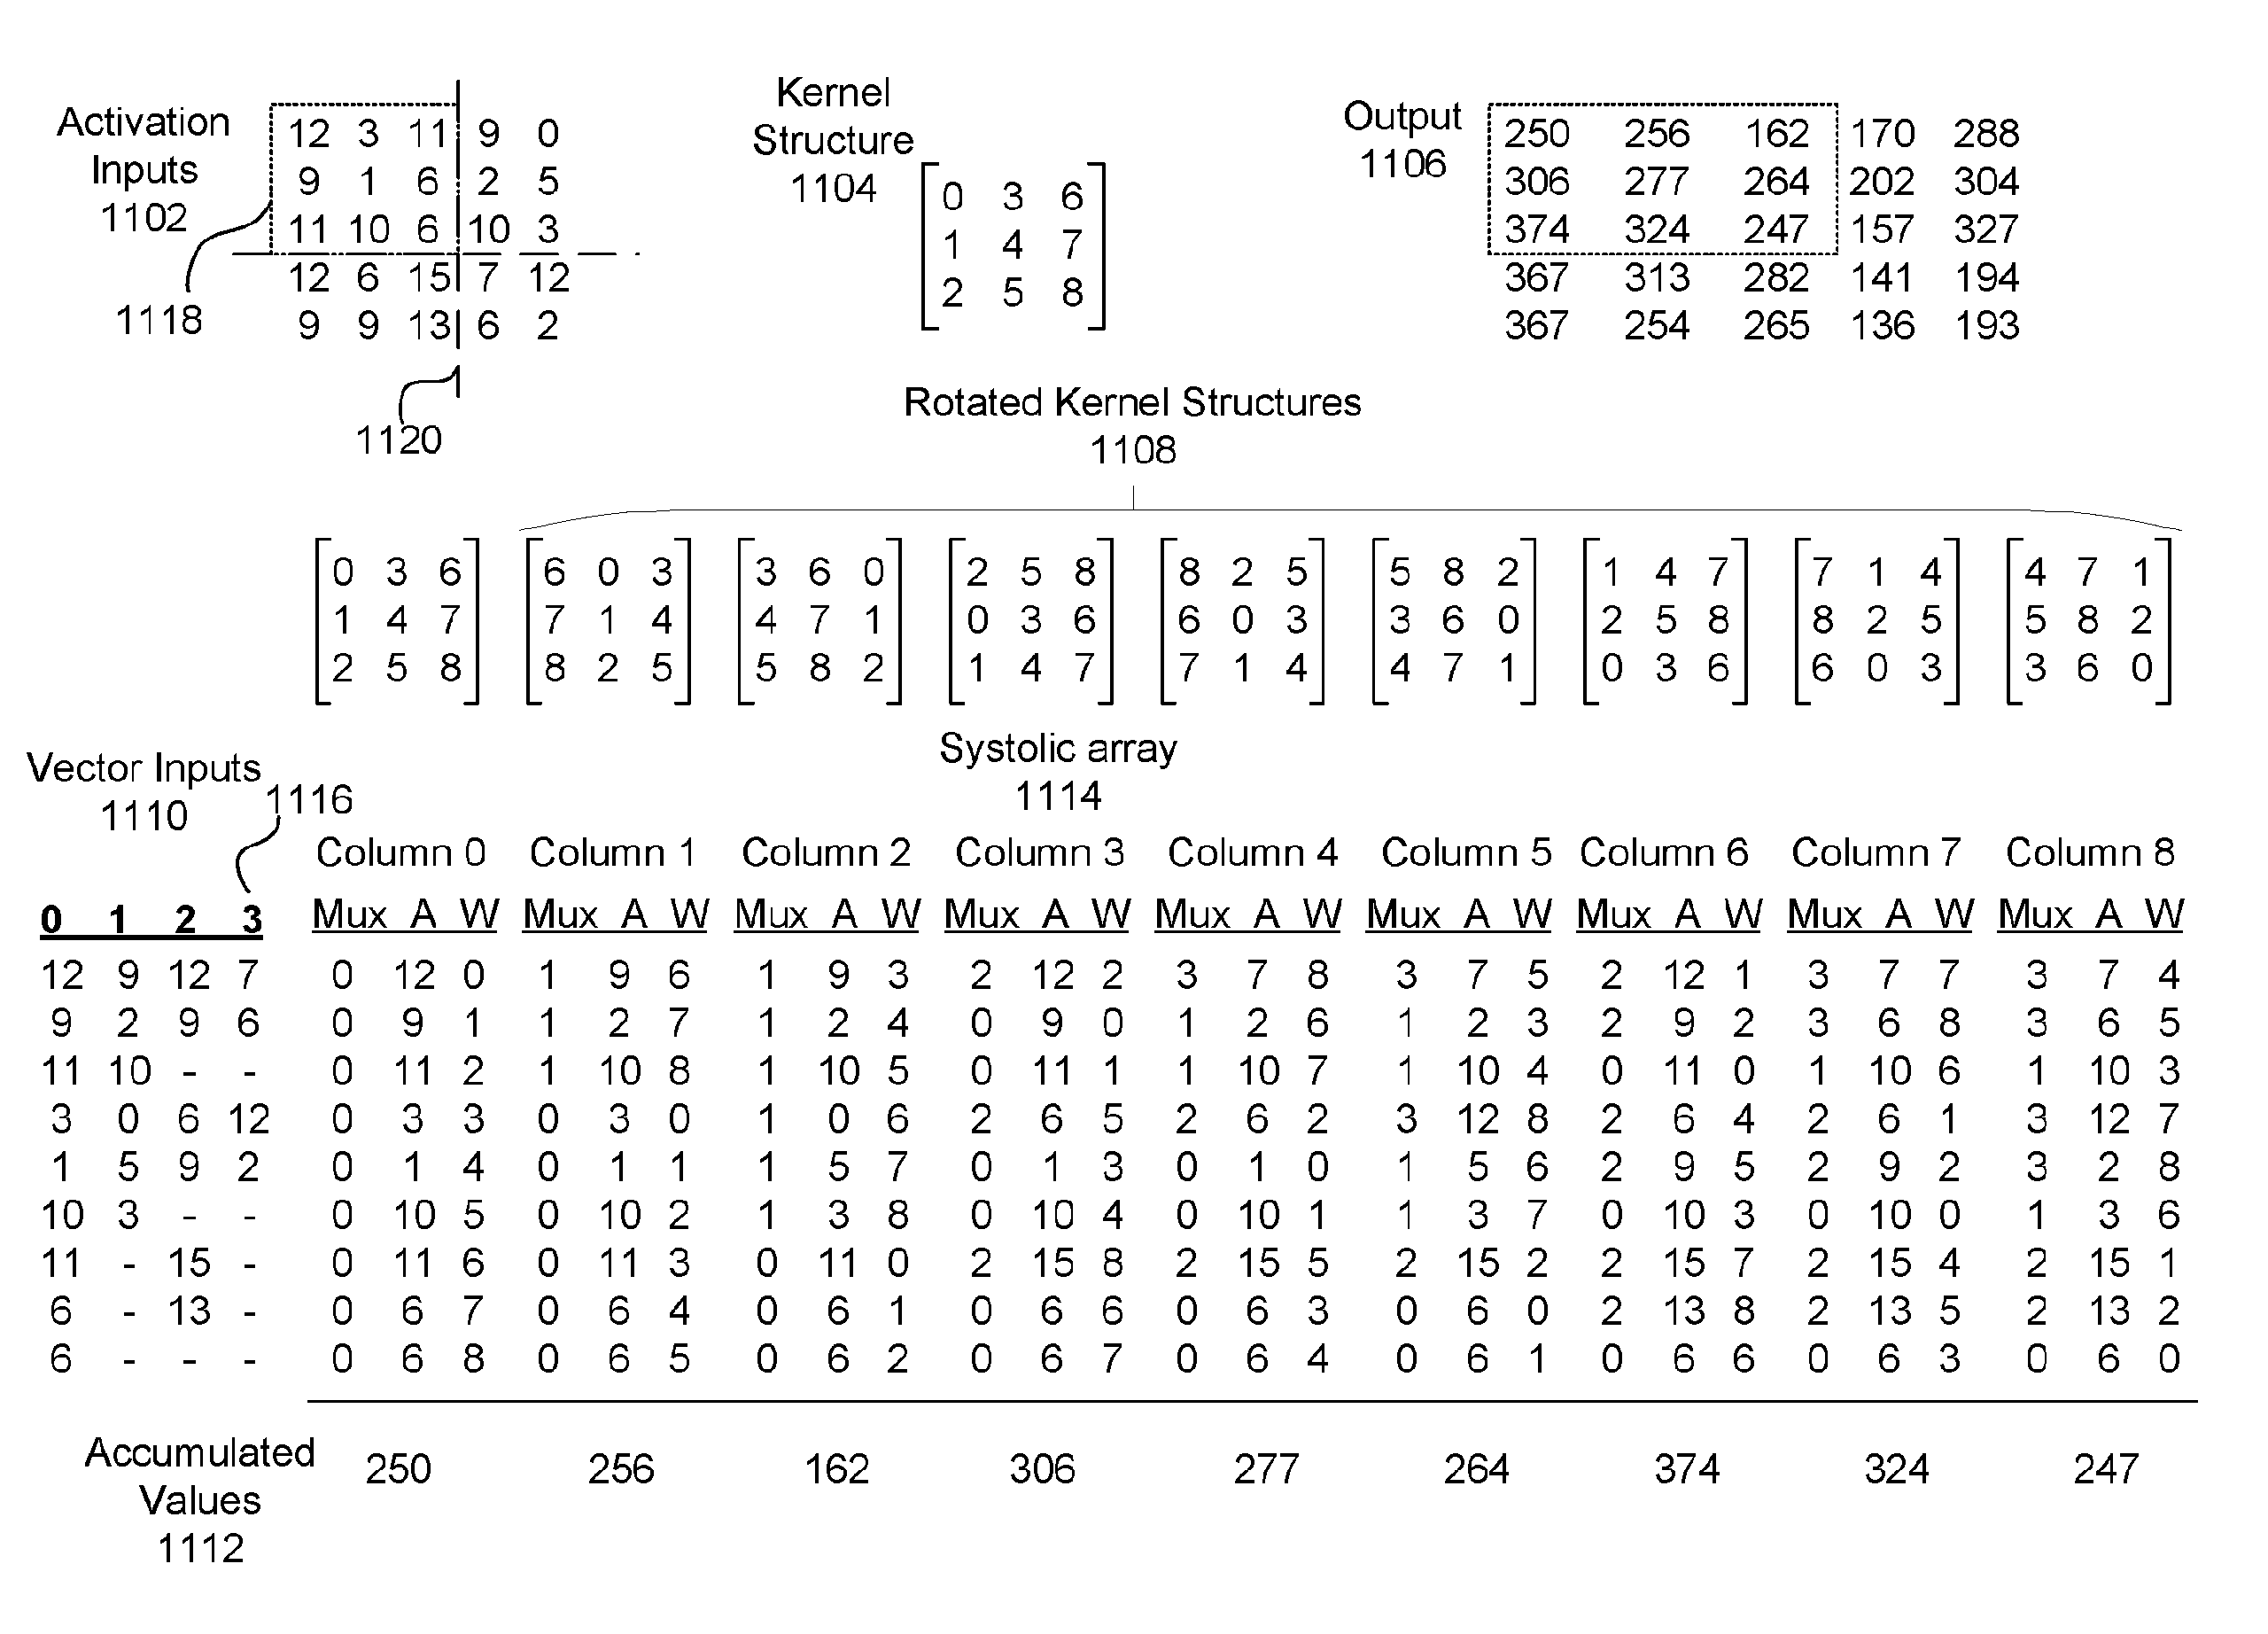
\includegraphics[width=15cm]{figures/tpu_systolic.png}
  \bicaption{TPU使用脉动阵列实例}{Example of TPU systolic array}
  \label{fig:tpu_systolic}
\end{figure}

